\\chapter{\\oner}\\label{one}\n\n\\begin{wrapfigure}{l}{0.05\\textwidth}\n\
\includegraphics[width=\\linewidth]{logo_1}\n\\label{fig:wrapfig}\n\\end{wrapfigure}\n\n\\paragraph{What is it?} The \\oner\\  is a malicious Android application masquerading as a plugin for a transportation application series developed by a South Korean developer. The series provides a range of information for each region of South Korea, such as bus stop locations, bus arrival times and so on.\n    \\section{VirusTotal}\n        \\begin{figure}[h]\n            \\centering\n            \
\includegraphics[width=1\\linewidth]{virustotal_1_summary.png}\n            \\caption{Virustotal summary analysis of file \\oner}\n            \\label{fig:virustotal_1_summary}\n        \\end{figure}\n        \\subsection{Detection}\n        \\begin{figure}\n            \\centering\n        \
\includegraphics[width=\\linewidth]{virustotal_1_detection_complete.png}\n            \\caption{VirusTotal Detection tab for \\oner}\n            \\label{fig:virustotal_1_detection_comp}\n        \\end{figure}\n        The antimalware analysis performed with VirusTotal, shown in fig. \\ref{fig:virustotal_1_detection_comp}, highlights that:\n        \\begin{itemize}\n            \\item 42 out of 76 security vendors flagged the file as \"\\textbf{malicious}\";\n            \\item 27 out of 76 security vendors flagged the file as a \"\\textbf{secure file}\";\n            \\item 7 out of 76 security vendors get a \"\\textbf{Unable to process file type}\" error\n        \\end{itemize}\n        \n        Most anti-malware programs correctly identify the sample as a generic android trojan, but some of them are even able to recognize its malware family (downloader). \n        A few vendors classify the sample as a generic android malware, without specifying the family nor the type (trojan).\\\\\n        It's interesting to notice that some famous vendor like Microsoft Defender, McAfee and Malwarebytes were unable to identify the file as malicious.\n         \\clearpage\n        \\subsection{Details}\n        \\begin{figure}[h]\n            \\centering\n            \
\includegraphics[width=.5\\linewidth]{virtustotal_first_permissions.png}\n            \\caption{Android Permission of \\oner}\n            \\label{fig:virustotal_first_permissions}\n        \\end{figure}\n            Here is an detailed analysis of the permissions (Fig. \\ref{fig:virustotal_first_permissions}) which are required by the APK, declared in the Manifest file (Fig. \\ref{fig:manifest_first}:\n\\begin{enumerate}\\label{sec:perm_analysis}\n\\item \\textbf{android.permission.ACCESS\\_FINE\\_LOCATION}$\\rightarrow$ Allows the precise location of the device (GPS, mobile networks, Wi-Fi).\n\\item  \\textbf{android.permission.ACCESS\\_COARSE\\_LOCATION}$\\rightarrow$ Provides approximate location (based on cellular towers and Wi-Fi).\n\\item \\textbf{android.permission.ACCESS\\_LOCATION\\_EXTRA\\_COMMANDS}$\\rightarrow$ Allows additional commands to be sent to the location provider (rarely used in legitimate apps).\n\\item  \\textbf{android.permission.READ\\_EXTERNAL\\_STORAGE}$\\rightarrow$ Allows reading files and data saved on external memory (photos, documents, downloads).\n\\item  \\textbf{android.permission.WRITE\\_EXTERNAL\\_STORAGE}$\\rightarrow$ Allows you to create or edit files on external storage.\n\\item  \\textbf{com.android.browser.permission.WRITE\\_HISTORY\\_BOOKMARKS}$\\rightarrow$ Allows editing of history and bookmarks in the stock Android browser.\n\\item  \\textbf{com.google.android.providers.gsf.permission.READ\\_GSERVICES}$\\rightarrow$ Reads Google Services Framework settings and data (e.g. device ID, GCM configurations).\n\\item  \\textbf{lmh.android.cwbus.permission.C2D\\_MESSAGE}$\\rightarrow$ Enable reception of cloud-to-device messages (C2DM/GCM/FCM).\n\\item  \\textbf{com.google.android.c2dm.permission.RECEIVE}$\\rightarrow$ Allows push notifications via Google Cloud Messaging (GCM/FCM).\n\\item  \\textbf{android.permission.INTERNET}$\\rightarrow$ Enables any network connection (HTTP, sockets, DNS).\n \\item  \\textbf{android.permission.ACCESS\\_NETWORK\\_STATE}$\\rightarrow$ Reads the status of network connections (Wi-Fi, mobile data).\n\\item  \\textbf{android.permission.ACCESS\\_WIFI\\_STATE}$\\rightarrow$ Gets information about Wi-Fi networks (SSID, BSSID, status).\n\\item  \\textbf{android.permission.CHANGE\\_WIFI\\_STATE}$\\rightarrow$ Changes Wi-Fi status (enable/disable, connects to networks).\n\\item  \\textbf{android.permission.WAKE\\_LOCK}$\\rightarrow$ Prevents the device from entering sleep mode.\n\\item  \\textbf{android.permission.VIBRATE }$\\rightarrow$ Controls the vibration engine.\n    \\end{enumerate}\n    \\begin{figure}\n        \\centering\n        \
\includegraphics[width=\\linewidth]{manifest_first.png}\n        \\caption{Android Manifest \\oner}\n        \\label{fig:manifest_first}\n    \\end{figure}\n            \n        \\subsection{Relations}\n        \\begin{figure}[h]\n            \\centering\n            \
\includegraphics[width=1\\linewidth]{first_relations.png}\n            \\caption{VirusTotal Relations Tab \\oner}\n            \\label{fig:virustotal_1_relations}\n        \\end{figure}\n         In addition, VirusTotal shows the contacted domains, URLs, and IP addresses associated with the APK, as shown in Fig. \\ref{fig:virustotal_1_relations}. The first three URLs are hosted on AWS Elastic Beanstalk (\\texttt{busappmanager.elasticbeanstalk.com}) and appear to retrieve the app category, runtime environment configuration, and remote download URL from a central database. This mechanism is consistent with \\emph{dropper-like} behaviour, as it allows the app to modify its functionality without requiring a new release. The fourth domain (\\texttt{gwk.adlibr.com/ad/config/init}) serves the advertising configuration and is still reachable; it responds only to POST requests, otherwise returning \\texttt{\\{ \"result\": 4003, \"message\": \"key\\_media\\_key\" \\}}. The bus-related domains (\\texttt{bus.changwon.go.kr}, \\texttt{openAPIs.changwon.go.kr}) are legitimate Korean public APIs, and no flagged domains were detected.\n        \\subsection{Behaviour}\n        VirusTotal's behaviour tab highlights several actions consistent with a suspicious application profile. The APK accesses file-related resources, builds JSON objects from file names and absolute paths, reads data into buffer streams, and opens files from absolute paths. It also shows the use of reflection/control to start another application from the current one, which may indicate dynamic or indirect execution of external components. In addition, the app interacts with advertising and analytics libraries, scheduling recording tasks and reading files from the assets directory. Overall, the observed behaviour suggests a complex application that performs file-system interaction and may support remote or dynamic actions rather than a simple bus-information client.\n        \n    \\section{Static Analysis}\n    Static analysis reveals that the application combines legitimate bus-related functionality with advertising SDKs, remote configuration mechanisms, native code, and update-like behavior. These elements suggest that the APK is not limited to its declared purpose, but may also support conditional execution and payload delivery at runtime.\n\n    \\subsection{MainActivity.java}\n\\begin{itemize}\n    \\item Inherits from \\texttt{BaseMainActivity}.\n    \\item Calls \\texttt{getTabView(BaseTabFragmentActivity.MainTabs.BUSTRANS).setVisibility(8)} to hide a UI tab.\n    \\item Provides ad network keys through \\texttt{getAdvertiseKey(...)}.\n    \\item Retrieves configuration via \\texttt{getEnvironmentProperties(...)}.\n\\end{itemize}\n\nThe analysis of \\texttt{MainActivity} suggests that the visible interface is partially controlled at runtime. In particular, the hiding of a UI tab and the retrieval of external configuration parameters indicate that the application may adapt its behavior dynamically depending on remotely supplied values. The use of multiple advertising providers such as AdMob, Facebook, and AdLib further confirms the presence of monetization-oriented logic.\n\n\\subsection{BaseMainActivity.java}\n\\begin{itemize}\n    \\item Acts as the central initialization hub.\n    \\item Loads the native library with \\texttt{System.loadLibrary(\"Audio3.0\")}.\n    \\item Declares and invokes the native methods \\texttt{startUpdate()} and \\texttt{updateApplication()}.\n    \\item Requests the runtime permissions:\n    \\begin{itemize}\n        \\item \\texttt{READ\\_EXTERNAL\\_STORAGE}\n        \\item \\texttt{WRITE\\_EXTERNAL\\_STORAGE}\n        \\item \\texttt{REQUEST\\_INSTALL\\_PACKAGES}\n    \\end{itemize}\n    \n    \\item Loads remote app environment data, including a URL, a database version, and a remote download URL.\n\\end{itemize}\n\nThis class is the most relevant part of the static analysis. The presence of a native library, together with methods related to update handling and the request for \\texttt{REQUEST\\_INSTALL\\_PACKAGES}, is consistent with dropper-like behavior. In addition, the remote environment loading mechanism allows the application to modify its behavior without requiring a new release.\n\n\\subsection{EnvConstant.java}\n\\begin{lstlisting}[language=Java]\npublic static final String ADAM_KEY = \"3034Z1OT1385cf1db09\";\npublic static final String ADLIB_KEY = \"590ea88a0cf2843c93807ed9\";\npublic static final String ADMOB_UNITID = \"ca-app-pub-0388605861855854/7499990747\";\npublic static final String FACEBOOK = \"627046304133735685335228304842\";\npublic static final String GA_TRACKER_ID = \"UA-56668425-6\";\n\\end{lstlisting}\n\nThe constants defined in this class confirm the integration of several advertising and analytics platforms. The presence of hardcoded keys is relevant from a security perspective, because it reduces transparency and can facilitate reverse engineering or unauthorized reuse of the embedded services. Although no endpoint URLs are directly visible in this file, the constants are consistent with the remote configuration logic observed in the main activity.\n\n\\subsection{BusApiWeb.java}\n\\begin{itemize}\n    \\item Makes calls to:\n    \\begin{itemize}\n        \\item \\texttt{http://bus.changwon.go.kr/busInfo/busInfoDetail.jsp}\n        \\item \\texttt{http://bus.changwon.go.kr/busInfo/mapLayer.jsp}\n    \\end{itemize}\n    \\item Uses Volley for networking.\n    \\item Parses HTML responses instead of JSON.\n    \\item Relays information through listeners.\n\\end{itemize}\n\nThe main issue in this component is the exclusive use of HTTP. Since the communication is not protected by TLS, bus stop identifiers and route data travel in plaintext and can be intercepted or modified in transit. This creates a clear man-in-the-middle risk and weakens the integrity of the information delivered by the application.\n\n\\subsection{AndroidManifest.xml}\n\\begin{itemize}\n    \\item Declares the following permissions:\n    \\begin{itemize}\n        \\item \\texttt{INTERNET}\n        \\item \\texttt{ACCESS\\_FINE\\_LOCATION}\n        \\item \\texttt{ACCESS\\_COARSE\\_LOCATION}\n        \\item \\texttt{READ\\_EXTERNAL\\_STORAGE}\n        \\item \\texttt{WRITE\\_EXTERNAL\\_STORAGE}\n        \\item \\texttt{REQUEST\\_INSTALL\\_PACKAGES}\n    \\end{itemize}\n    \\item Declares multiple ad and analytics activities:\n    \\begin{itemize}\n        \\item AdLib\n        \\item AdMob\n        \\item Facebook\n        \\item AdFit (Kakao)\n    \\end{itemize}\n    \\item Includes GCM and Firebase messaging support.\n    \\item Declares the custom service \\texttt{lmh.android.cwbus.GCMIntentService}.\n\\end{itemize}\n\nThe manifest confirms that the application can receive background messages and interact with external services. In particular, the presence of \\texttt{REQUEST\\_INSTALL\\_PACKAGES} is significant because, if granted, it may allow silent installation of additional APKs. Combined with GCM/Firebase messaging, this suggests the possibility of remote triggering of behavior.\n\n\\subsection{AppInfoActivity.java}\n\\begin{itemize}\n    \\item Displays the link \\texttt{http://bus.changwon.go.kr/main}.\n    \\item Serves to legitimize the app.\n    \\item Contains no interaction logic.\n\\end{itemize}\n\nThis activity appears to be mainly cosmetic, since it exposes a public bus-related URL while providing no additional functional logic. Its role seems to be presenting the application as a legitimate transportation service, even though the rest of the static analysis reveals a much more complex and suspicious architecture.\n\n\\section{Summary}\n\n\\begin{longtable}{|p{0.45\\textwidth}|p{0.45\\textwidth}|}\n\\hline\n\\textbf{Suspicious Pattern} & \\textbf{Explanation} \\\\\n\\hline\nMultiple ad SDKs & Monetization through aggressive advertising and possible ad fraud. \\\\\n\\hline\nNative libraries (JNI) & Executes code not visible to standard Java analysis tools. \\\\\n\\hline\n\\texttt{REQUEST\\_INSTALL\\_PACKAGES} & Suggests dropper-like behavior and possible APK installation without market interaction. \\\\\n\\hline\nUnencrypted HTTP endpoints & Data can be intercepted or modified through MITM attacks. \\\\\n\\hline\nDynamic configuration via \\texttt{getEnvironmentProperties(...)} & The app can change behavior based on remote values. \\\\\n\\hline\nFragment and tab visibility manipulation & Suggests conditional or delayed functionality and may hide behavior from users and analysts. \\\\\n\\hline\n\\end{longtable}\n    \\section{MobSF}\n\\begin{figure}[h]\n    \\centering\n    \
\includegraphics[width=\\linewidth]{mobsf_one_scorecard.png}\n    \\caption{MobSF Scorecard \\oner}\n    \\label{fig:mobsf_scorecard_one}\n\\end{figure}\nMobSF highlights several security issues in the analyzed APK, confirming that the application exposes a broad attack surface. In particular, the scorecard shows problems related to signature schemes, outdated Android compatibility, exported components, insecure storage, and the presence of multiple privacy trackers.\n\n\\subsection{Certificate Analysis}\nDuring the analysis, MobSF identified one unique certificate. The binary is signed only with the v1 signature scheme, while v2, v3, and v4 are not present. The certificate uses \\texttt{SHA1withRSA}, with the following subject and issuer: \\texttt{C=ko, L=Jeonju, CN=Myoung-Hun Lee}. Since the app relies on a legacy signing scheme and a weak hash algorithm, it is exposed to known cryptographic and platform-level weaknesses.\n\n\\subsection{High Severity Findings}\nMobSF reports nine high-severity issues. The first one is the vulnerability to the Janus attack, because the application is signed only with the v1 scheme. The second is the use of SHA-1, which is vulnerable to hash collision attacks. The third is the low minimum SDK version (\\texttt{minSdk=14}), which allows installation on older Android versions with unresolved vulnerabilities. MobSF also detects Android Task Hijacking and StrandHogg weaknesses in \\texttt{lmh.android.cwbus.activity.AlarmActivity} and in \\texttt{com.google.android.gms.appinvite.PreviewActivity}. In addition, the analysis flags debug configuration, weak encryption in the AdLib library, a world-readable file or shared preference, and the presence of more than eight privacy trackers.\n\n\\subsection{Medium Severity Findings}\nThe medium-severity findings are mainly related to insecure configuration and component exposure. The flag \\texttt{android:allowBackup=true} makes the application data backup accessible through ADB when USB debugging is enabled. Several activities and receivers are exported or not properly protected, including \\texttt{AlarmActivity}, \\texttt{CampaignTrackingReceiver}, \\texttt{FirebaseMessagingService}, \\texttt{TagManagerPreviewActivity}, and Firebase/GCM-related components. MobSF also warns about the external permission associated with \\texttt{INSTALL\\_PACKAGES}, which is particularly relevant because it may support silent installation behavior.\n\nThe scan also identifies insecure storage and code-quality issues. The application can read and write external storage, which exposes data to other apps on the device. MobSF further detects hardcoded secrets in multiple files, insecure WebView usage, temporary file creation, an insecure random number generator, possible SQL injection through raw queries, and the use of MD5, which is considered weak due to collision resistance problems.\n\n\\subsection{Low Severity Findings}\nMobSF reports one informational issue: the application logs information, including potentially sensitive data. It also reports two secure findings: the use of SSL communication and the presence of root detection capabilities. Finally, the scorecard flags one hotspot related to a critical permission, reinforcing the idea that the app is highly sensitive from a security perspective.\n\n\\subsection{Overall Assessment}\nOverall, MobSF confirms that the APK is not a simple transportation application. The combination of weak signing, exported components, insecure storage, dynamic installation capabilities, and ad/tracking infrastructure suggests an application with a high security risk and behavior consistent with a trojanized or heavily repurposed app.\n    \\section{Genymotion}\n\nThe dynamic analysis performed in Genymotion provided practical confirmation of several findings obtained during static inspection. The application interacts with remote endpoints, relies on advertising frameworks, and appears capable of adapting part of its behavior through external configuration data rather than through local code changes.\n\nThis behavior is relevant because it indicates that the app is not limited to a simple transportation interface. Instead, it combines user-facing functionality with background services, ad-related activity, and network-driven logic, which is consistent with a repackaged or trojanized application structure.\n\nThe emulator analysis therefore strengthens the overall assessment of the sample as suspicious. In combination with the insecure HTTP traffic, exported components, hardcoded secrets, and multiple privacy trackers identified by other tools, the Genymotion observations support the conclusion that the APK presents a non-negligible security risk.\n\\begin{figure}[htbp]\n    \\centering\n    \\begin{subfigure}[t]{0.48\\linewidth}\n        \\centering\n        \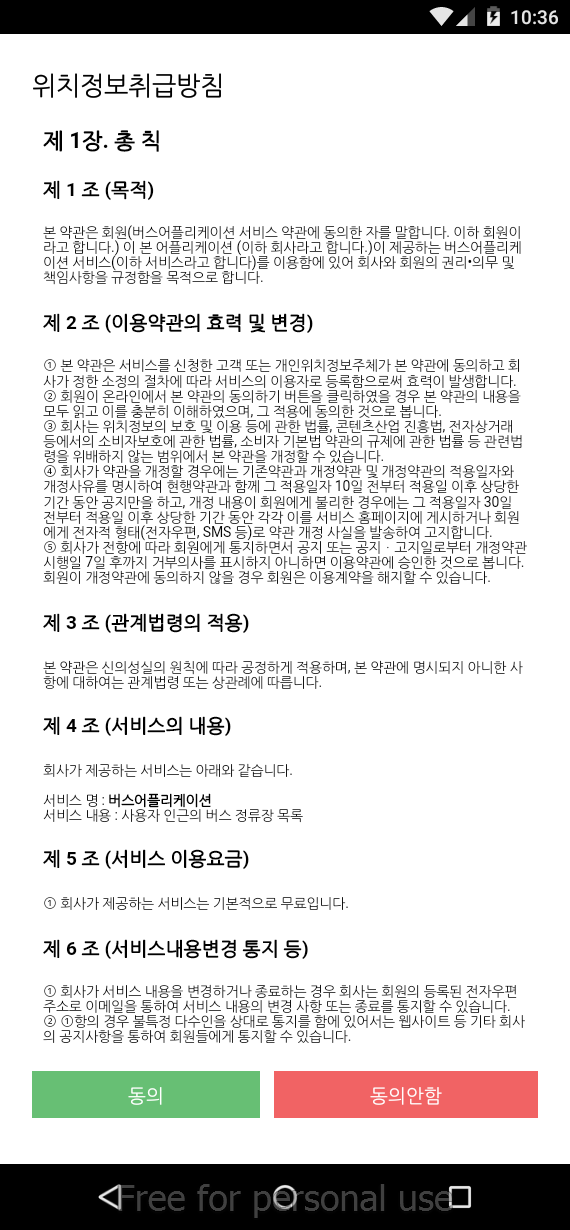
\includegraphics[width=0.68\\linewidth]{img/apk_1/screenshots/screenshot-2026-06-26_16.36.35.339.png}\n        \\caption{Privacy policy / consent screen shown at app startup \\oner}\n        \\label{fig:genymotion-1}\n    \\end{subfigure}\n    \\hfill\n    \\begin{subfigure}[t]{0.48\\linewidth}\n        \\centering\n        \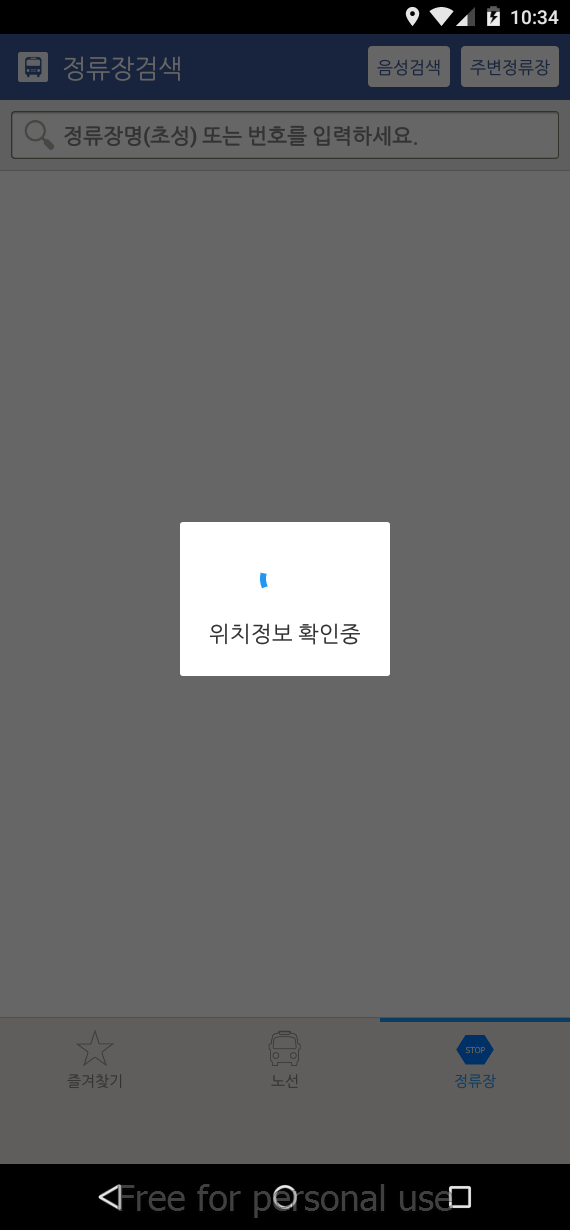
\includegraphics[width=0.68\\linewidth]{img/apk_1/screenshots/screenshot-2026-06-26_16.34.31.953.png}\n        \\caption{Runtime location verification screen in Genymotion \\oner}\n        \\label{fig:genymotion-2}\n    \\end{subfigure}\n\n    \\vspace{0.5cm}\n\n    \\begin{subfigure}[t]{0.48\\linewidth}\n        \\centering\n        \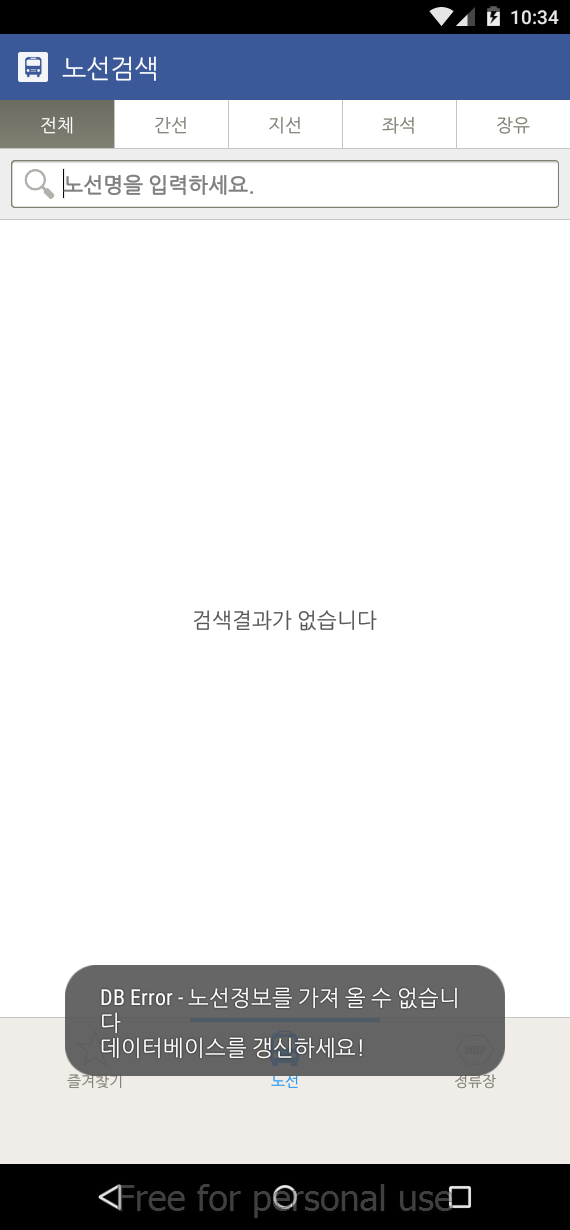
\includegraphics[width=0.68\\linewidth]{img/apk_1/screenshots/screenshot-2026-06-26_16.34.18.192.png}\n        \\caption{Main bus search screen showing the DB error during dynamic analysis \\oner}\n        \\label{fig:genymotion-3}\n    \\end{subfigure}\n    \\hfill\n    \\begin{subfigure}[t]{0.48\\linewidth}\n        \\centering\n        \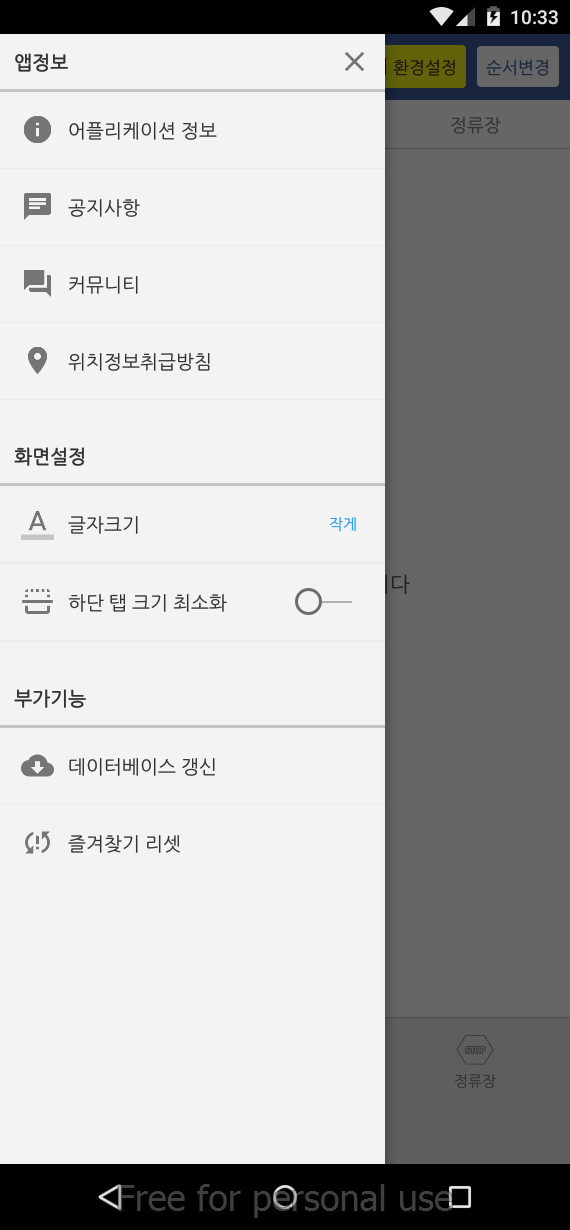
\includegraphics[width=0.68\\linewidth]{img/apk_1/screenshots/screenshot-2026-06-26_16.33.06.863.png}\n        \\caption{Side menu with maintenance options such as database refresh and favorites reset \\oner}\n        \\label{fig:genymotion-4}\n    \\end{subfigure}\n\n    \\caption{Genymotion dynamic analysis screenshots of \\oner}\n    \\label{fig:genymotion-grid}\n\\end{figure}\n\\section{Conclusion}\n\nThe combined results of VirusTotal, static analysis, MobSF, and Genymotion consistently indicate that the analyzed APK is suspicious and potentially malicious. Across the different tools, the same core patterns emerge: unencrypted network traffic, aggressive use of advertising libraries, remote configuration, exported components, and several weaknesses related to storage and cryptography.\n\nThe static inspection shows that the application is not limited to a simple bus-information interface. Instead, it includes native code, runtime permissions for package installation, hidden or manipulated UI behavior, and remote update logic, all of which are typical indicators of repackaged or dropper-like software.\n\nMobSF strengthens this conclusion by reporting a large number of high- and medium-severity issues, including Janus vulnerability exposure, SHA-1 signing, StrandHogg weaknesses, hardcoded secrets, world-readable files, insecure WebView usage, and multiple privacy trackers. In parallel, the dynamic analysis in Genymotion confirms that the app interacts with remote services and relies on background components and advertising frameworks, supporting the idea that some behavior is driven at runtime rather than being fully visible from static inspection.\n\nOverall, the APK should be treated as unsafe. Even if part of its visible functionality appears legitimate, the combination of insecure communication, suspicious permissions, and evasive implementation choices shows a clear mismatch between the declared purpose of the app and its actual security posture.\n